\subsection{Segmentation of Echocardiography Frames}

For the first part of this body of work, we develop a baseline segmentation
accuracy when segmenting echo frames using an encoder-decoder neural network.
For our work, we used the well-known U-Net architecture. \newline

For all the experiments in this work, we used the CAMUS datast
\cite{leclercDeepLearningSegmentation2019} which was also the dataset behind the
C-GAN work of Abdi et al. All of the experiments were run using Python 3 and
TensorFlow 2.1.0. All of our code is available on GitHub at
https://github.com/hewittwill/CS380 \newline

The CAMUS dataset was downloaded and converted from .MHD/.RAW format to a NumPy
array using the SimpleITK library for Python. Apical 2 Chamber (A2C) frames at
ES and ED (only the ground truth for ES and ED is provided) were extracted,
resampled to 256x256 and pixel values normalised to 0-1. All preprocessing steps
were carried out using NumPy and OpenCV \newline

The final dataset to establish baseline performance consisted of 900 samples,
split 80:10:10 for train:test:validation (720, 90, 90 samples respectively). \newline

We built a U-Net encoder-decoder segmentation neural network that used the
pretrained (on ImageNet) VGG-16 model from Keras. The last convolution block was
dropped, and the weights for the encoder frozen (this was saved as a
hyperparameter). Transpose convolutional layers were used for upsampling, and
skip connections were additionally used. The overall model architecture can be
seen in Figure \ref{fig:unet}. \newline


\begin{figure}[H]
    \centering
    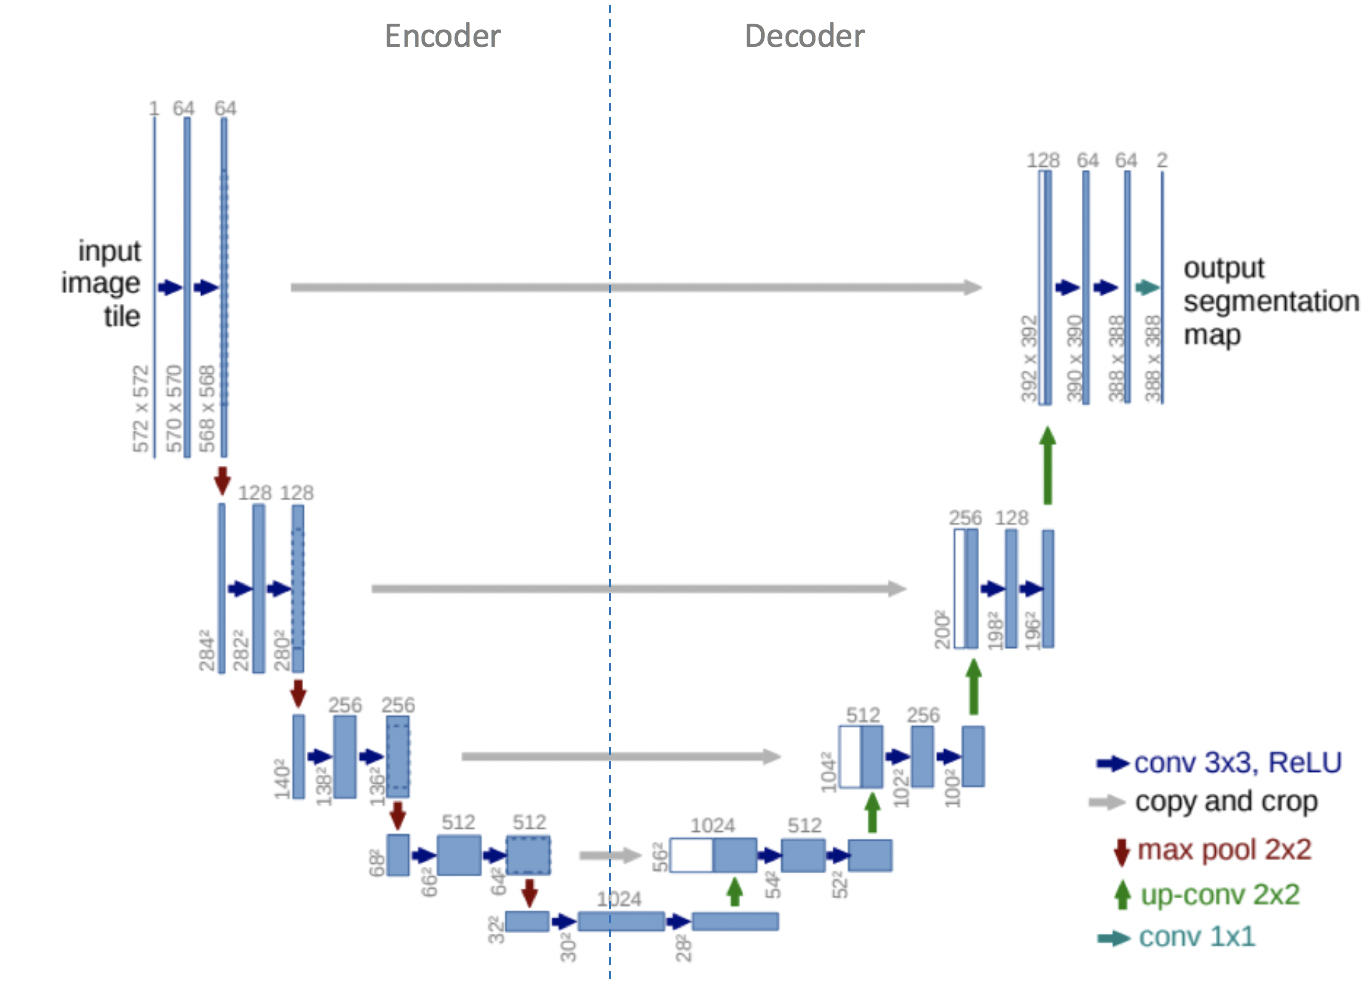
\includegraphics[width=1.0\textwidth]{figures/unet.png}
    \caption{U-Net architecture used in this study, Credit: Ronneberger et al. \cite{ronneberger2015u}}
    \label{fig:unet}
\end{figure}


For training the Adam optimizer was used, with a base learning rate of 1e-5.
Weighted Categorical Cross Entropy (WCCE) was used for a loss function, the
weighting applied to each class was roughly proportional to its prevalence in
the image. Dropout was applied in the bottleneck layers, baseline dropout
threshold of 0.5. The model was trained on a batch size of 16. Convergence
was subjectively defined as when validation loss began increasing
over training loss. \newline

The model was evaluated on a seperate test dataset, which was not encountered
during training time. There was 90 samples in the test dataset. \newline

\subsection{Validating C-GANs for Echocardiography Frames}

For our purposes, it was of interest to see if a C-GAN could be trained that
would be able to generate photorealistic echocardiography frames from a
segmentation mask input condition. \newline

We used just ED frames from A2C views in the CAMUS dataset, which were
preprocessed similarly to in the segmentation step, resampled to 256x256 and
normalised to have pixel values from [0-1]. \newline

We used the same framework as Abdi et al. to train a C-GAN on ED frames of the
A2C view. The network was trained for 100,000 epochs with the model and
sample images saved every 100 epochs. The Adam optimizer was used, with a
learning rate of 1.3e-4 and 1.5e-4 for the generator and discriminator
respectively. Patch size was set to 16x16 for the patch based discriminator, and
batch size was set to 8.\newline

\subsection{Data Augmentation for the Segmentation of Echocardiography Frames}

To compare the effect on segmentation accuracy for our two data augmentation
techniques, we created two new dataset labelled "real" and "generated". Real
contained the original CAMUS training dataset with elastic deformation applied
directly to images and their segmentation mask. Generated contained synthetic
images produced by passing the same deformed segmentation mask as in the real
dataset, to the generator trained in 3.2.
\newline

Elastic deformations for both datasets were created using the elasticdeform
library for Python. Each dataset contained the original ground truth images, as well
as a deformed counterpart to each image giving double the original dataset size. In total,
each dataset contained 1800 images. \newline

Two seperate U-Net models were trained using the same framework as 3.1, with the
same hyperparameters and number of epochs as the baseline. This was enforced to
give a good objective view of the effect of the different augmentation methods,
and to isolate the effect on the accuracy of the model to just the independent
variable (type of data augmentation). \newline

The models were both tested on the same test dataset as the baseline, which was
not encountered during training time. No elastic deformations were applied to
the testing dataset. 